
\section{Continuous Latent Diffusion Language Model}

This section first presents \method as a hierarchical latent-variable language model with a rigorous probabilistic definition. We also outline the overall workflow of \method. We then place \method in a unified theoretical framework together with AR models, discrete denoising language models, and continuous token-space methods. Detailed derivations and proofs are deferred to Appendices~\ref{app:prob_model}, \ref{app:inference_and_likelihood}, \ref{app:comparison} and \ref{app:advantages}.

\subsection{Theoretical Foundations of Cola DLM}

In this subsection, we present \method as a hierarchical latent-variable language model with a rigorous probabilistic definition. We then introduce its unconditional and conditional probability estimators. Detailed derivations and proofs are provided in Appendices~\ref{app:prob_model} and~\ref{app:inference_and_likelihood}.

\subsubsection{Theoretical Formulation of Cola DLM}

\paragraph{\textbf{Hierarchical latent-variable modeling.}}
Let \(x \in \mathcal X\) denote a discrete text sequence, and let \(z_0 \in \mathbb R^d\) denote its continuous latent variable. The generative model of \method consists of a conditional decoder \(p_\theta(x \mid z_0)\) and a latent prior \(p_\psi(z_0)\):
\begin{equation}
p(x,z_0)=p_\theta(x\mid z_0)\,p_\psi(z_0),
\qquad
p(x)=\int p_\theta(x\mid z_0)\,p_\psi(z_0)\,dz_0.
\label{eq:main_ldlm_joint}
\end{equation}
Here, \(q_\phi(z_0\mid x)\) is used only for variational inference during training, and is not part of the generative model itself.

We model \(p_\psi(z_0)\) with a continuous-flow prior. Let the base distribution be \(p_1(z_1)=\mathcal N(0,I)\), and let \(v_\psi(z_t,t)\) be the vector field. Then
\begin{equation}
z_1\sim p_1,\qquad
\frac{dz_t}{dt}=v_\psi(z_t,t),\qquad
z_0=\Phi^\psi_{0\leftarrow 1}(z_1),
\label{eq:main_cnf_prior}
\end{equation}
which induces \(p_\psi=(\Phi^\psi_{0\leftarrow 1})_\sharp p_1\). In the sequence implementation, the latent is further decomposed into blocks, \(z_0=(z_0^{(1)},\ldots,z_0^{(B)})\), with
\begin{equation}
p_\psi(z_0)=p_\psi(z_0^{(1)})\prod_{b=2}^{B}p_\psi(z_0^{(b)}\mid z_0^{(<b)}).
\label{eq:main_block_prior}
\end{equation}
This factorization directly corresponds to the block-causal prior learning and block-wise inference used later.

\paragraph{\textbf{ELBO and prior learning.}}
By Jensen's inequality, the training lower bound of \method is
\begin{equation}
\log p(x)\ge
\mathbb E_{q_\phi(z_0\mid x)}
\!\left[
\log p_\theta(x\mid z_0)+\log p_\psi(z_0)-\log q_\phi(z_0\mid x)
\right]
=: \mathcal L_{\mathrm{ELBO}}(x).
\label{eq:main_elbo}
\end{equation}
Training therefore maximizes \(\mathcal L_{\mathrm{ELBO}}(x)\), or equivalently minimizes \(-\mathcal L_{\mathrm{ELBO}}(x)\).

Let the aggregated posterior be \(\bar q_\phi(z_0)=\int q_\phi(z_0\mid x)\,\pdata(x)\,dx\). The expected ELBO can then be written as
\begin{equation}
\mathbb E_{\pdata(x)}[\mathcal L_{\mathrm{ELBO}}(x)]
=
\mathbb E_{q(x,z_0)}[\log p_\theta(x\mid z_0)]
-
I_q(X;Z_0)
-
\KL(\bar q_\phi(z_0)\,\|\,p_\psi(z_0)),
\label{eq:main_avg_elbo}
\end{equation}
where \(q(x,z_0)=\pdata(x)q_\phi(z_0\mid x)\). This decomposition shows that \method separates text modeling into conditional reconstruction, information compression, and prior matching.

When the encoder and decoder are fixed, prior learning reduces to
\begin{equation}
\max_\psi\ \mathbb E_{z_0\sim \bar q_\phi}[\log p_\psi(z_0)]
\quad\Longleftrightarrow\quad
\min_\psi\ \KL(\bar q_\phi(z_0)\,\|\,p_\psi(z_0)).
\label{eq:main_prior_subproblem}
\end{equation}
In practice, we do not optimize the density directly. Instead, we learn the corresponding vector field with Flow Matching. For block \(b\), the conditional FM objective is
\begin{equation}
\mathcal L_{\mathrm{FM}}
=
\sum_{b=1}^{B}
\mathbb E_{t,z_0,z_1}
\left[
\left\|
v_\psi\!\bigl(z_t^{(b)},t;z_0^{(<b)}\bigr)-u_t^{(b)}(z_0,z_1)
\right\|_2^2
\right].
\label{eq:main_fm}
\end{equation}
Flow Matching is therefore a solver for the prior in \method, rather than the definition of the model itself.

\obsbox{
\textbf{Summary.}
The generative distribution of \method is defined by the hierarchical factorization in Eq.~\eqref{eq:main_ldlm_joint}: the latent prior \(p_\psi(z_0)\) generates global continuous semantics, and the decoder \(p_\theta(x\mid z_0)\) realizes discrete text. The encoder \(q_\phi(z_0\mid x)\) is not part of the generative model, but an inference model that lifts the observed data distribution \(\pdata(x)\) into a model-dependent latent joint distribution,
\[
q_\phi(x,z_0)=\pdata(x)q_\phi(z_0\mid x),
\qquad
\bar q_\phi(z_0)=\int q_\phi(z_0\mid x)\pdata(x)\,dx.
\]
Thus, while \(\pdata(x)\) is fixed, the induced latent distribution \(\bar q_\phi\) is not. When the representation is fixed, prior learning fits \(p_\psi\) to \(\bar q_\phi\). Under joint training, however, \(\bar q_\phi\) and \(p_\psi\) co-evolve: the encoder reshapes the latent data distribution, while the learned prior regularizes and organizes the latent space. Flow Matching is therefore only an implementation choice for learning this prior transport; the underlying model remains a hierarchical latent-variable language model.
}

\begin{figure}[t]
\centering

\begin{minipage}[t][0.185\textheight][t]{0.485\linewidth}
\vspace{0pt}
\footnotesize
\begin{sidealgorithm}{alg:uncond_loglik}{Unconditional log-likelihood estimation}
\Require $x$, $K$
\For{$k = 1,\dots,K$}
    \State sample $z_0^{(k)} \sim q_\phi(z_0 \mid x)$
    \State $w^{(k)} \gets \log p_\theta(x \mid z_0^{(k)}) + \log p_\psi(z_0^{(k)})$
    \Statex \hspace{\algorithmicindent}$\qquad\quad - \log q_\phi(z_0^{(k)} \mid x)$
\EndFor
\State output $\log \widehat p_{\mathrm{ELBO}}(x)=\frac{1}{K}\sum_{k=1}^K w^{(k)}$
\Statex \hspace{\algorithmicindent}or $\log \widehat p_{\mathrm{IWAE}}(x)=\log \frac{1}{K}\sum_{k=1}^K \exp(w^{(k)})$
\Statex \hspace{\algorithmicindent}according to Eq.~\eqref{eq:main_p_estimators}
\end{sidealgorithm}
\end{minipage}
\hfill
\begin{minipage}[t][0.185\textheight][t]{0.485\linewidth}
\vspace{0pt}
\footnotesize
\begin{sidealgorithm}{alg:cond_loglik}{Conditional log-likelihood estimation}
\Require $x_{\mathrm{pre}}$, $x_{\mathrm{res}}$
\State estimate $\log \widehat p(x_{\mathrm{pre}},x_{\mathrm{res}})$
\Statex \hspace{\algorithmicindent}using Algorithm~\ref{alg:uncond_loglik}
\State estimate $\log \widehat p(x_{\mathrm{pre}})$
\Statex \hspace{\algorithmicindent}using Algorithm~\ref{alg:uncond_loglik}
\State \Return $\log \widehat p(x_{\mathrm{res}} \mid x_{\mathrm{pre}})$
\Statex \hspace{\algorithmicindent}$= \log \widehat p(x_{\mathrm{pre}},x_{\mathrm{res}}) - \log \widehat p(x_{\mathrm{pre}})$
\Statex \hspace{\algorithmicindent}according to Eq.~\eqref{eq:main_cond_estimator}
\end{sidealgorithm}
\end{minipage}

\end{figure}
\subsubsection{Probability Estimation for Cola DLM}

\paragraph{\textbf{Unconditional probability estimation.}}
At evaluation time, we approximate \(\log p(x)\). For samples \(z_0^{(k)}\sim q_\phi(z_0\mid x)\), define the importance weight
\begin{equation}
\log w^{(k)}
=
\log p_\theta(x\mid z_0^{(k)})
+\log p_\psi(z_0^{(k)})
-\log q_\phi(z_0^{(k)}\mid x).
\label{eq:main_importance_weight}
\end{equation}

The prior term \(\log p_\psi(z_0^{(k)})\) is evaluated by the CNF change-of-variables formula. Concretely, we solve the augmented ODE
\begin{equation}
\frac{\dd}{\dd t}
\begin{bmatrix}
z_t \\
\ell_t
\end{bmatrix}
=
\begin{bmatrix}
\vv_{\psi}(z_t,t) \\
\nabla\!\cdot \vv_{\psi}(z_t,t)
\end{bmatrix},
\qquad
\begin{bmatrix}
z_0 \\
\ell_0
\end{bmatrix}
=
\begin{bmatrix}
z_0^{(k)} \\
0
\end{bmatrix},
\label{eq:main_augmented_ode}
\end{equation}
from \(t=0\) to \(t=1\), yielding \((z_1^{(k)},\ell_1^{(k)})\). We then obtain
\begin{equation}
\log p_\psi(z_0^{(k)})
=
\log p_1(z_1^{(k)})+\ell_1^{(k)},
\label{eq:main_prior_eval}
\end{equation}
where \(p_1\) is the terminal base distribution. In high dimensions, the divergence term is estimated with Hutchinson's trace estimator:
\begin{equation}
\nabla\!\cdot \vv_{\psi}(z_t,t)
=
\mathrm{Tr}\!\left(\frac{\partial \vv_{\psi}(z_t,t)}{\partial z_t}\right)
\approx
\veps^{\top}
\frac{\partial \vv_{\psi}(z_t,t)}{\partial z_t}
\veps,
\qquad
\veps\sim\mathcal N(0,I),
\label{eq:main_hutchinson}
\end{equation}
where the same \(\veps\) is fixed within one ODE solve.

This gives two standard estimators, namely the ELBO-style and IWAE-style estimators:
\begin{equation}
\log \widehat p_{\mathrm{ELBO},K}(x)
=
\frac{1}{K}\sum_{k=1}^{K}\log w^{(k)},
\qquad
\log \widehat p_{\mathrm{IWAE},K}(x)
=
\log\!\left(\frac{1}{K}\sum_{k=1}^{K}e^{\log w^{(k)}}\right).
\label{eq:main_p_estimators}
\end{equation}
The IWAE-style estimator is typically tighter.

\paragraph{\textbf{Conditional probability estimation.}}
For a prefix--response decomposition \(x=(x_{\mathrm{pre}},x_{\mathrm{res}})\), the exact identity is
\begin{equation}
\log p(x_{\mathrm{res}}\mid x_{\mathrm{pre}})
=
\log p(x_{\mathrm{pre}},x_{\mathrm{res}})
-
\log p(x_{\mathrm{pre}}).
\label{eq:main_cond_identity}
\end{equation}
We therefore obtain a plug-in estimator by scoring the joint sequence and the prefix with the same unconditional estimator:
\begin{equation}
\log \widehat p(x_{\mathrm{res}}\mid x_{\mathrm{pre}})
=
\log \widehat p(x_{\mathrm{pre}},x_{\mathrm{res}})
-
\log \widehat p(x_{\mathrm{pre}}).
\label{eq:main_cond_estimator}
\end{equation}

\subsection{Workflow of Cola DLM}
In this section, we describe the overall workflow of \method in detail. As illustrated in Figure~\ref{fig:cola_main_fig}, we explain the method from three perspectives: the pretraining of the Text VAE, the pretraining of prior learning with the Text DiT, and the inference process of \method.
\subsubsection{Text VAE Pretraining}

In the first stage, we learn a stable latent--text correspondence. The encoder maps text into the latent space, and the decoder reconstructs the original text conditioned on the latent:
\begin{equation}
z_0\sim q_\phi(z_0\mid x),
\qquad
\hat x\sim p_\theta(x\mid z_0).
\label{eq:main_stage1_io}
\end{equation}
The goal of this stage is not to learn the final prior, but to establish a stable division of labor between information stored in the latent and information recovered by the decoder.

The corresponding objective is
\begin{equation}
\mathcal L_{\mathrm{VAE}}
=
-\mathbb E_{q_\phi(z_0\mid x)}\log p_\theta(x\mid z_0)
+\beta\,\KL(q_\phi(z_0\mid x)\,\|\,p_{\mathrm{base}}(z_0))
+\lambda_{\mathrm{mask}}\mathcal L_{\mathrm{mask}}.
\label{eq:main_stage1_loss}
\end{equation}
Here, \(\mathcal L_{\mathrm{mask}}\) is the BERT-style masking loss shown in the figure. It prevents the VAE encoder from collapsing semantically while the decoder merely memorizes surface text. In our experiments, the VAE does not compress the sequence length. To prevent information leakage and facilitate subsequent streaming generation, both our VAE encoder and decoder are strictly causal.

\begin{figure}[t]
    \centering
    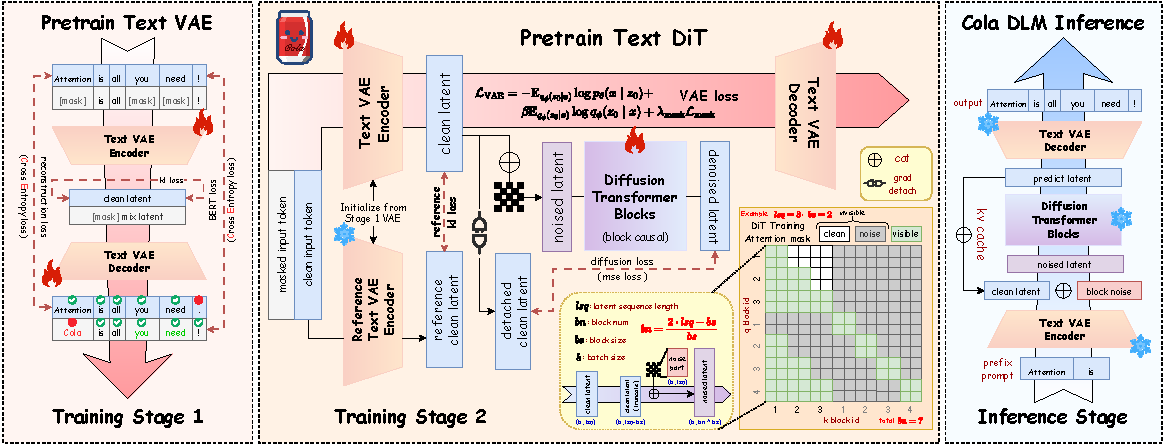
\includegraphics[width=1\textwidth]{fig/cola_main_fig.pdf}
    \caption{\textbf{The Overall Workflow of Cola DLM.} Detailed illustration of the training and inference pipeline of \method. \emph{Training Stage 1} shows Text VAE pretraining with reconstruction, BERT, and KL losses. \emph{Training Stage 2} shows joint pretraining of the Text VAE and Text DiT with gradient control for stable optimization, where a specialized block-causal mechanism is adopted in the DiT. \emph{Inference Stage} illustrates the decoding process with KV cache.}
    \label{fig:cola_main_fig}
\end{figure}

\subsubsection{Prior Learning with Block-Causal DiT}

In the second stage, we learn a conditional prior on the stabilized latent space. For block \(b\), the visible set consists of the historical clean latent blocks and the current noisy block:
\begin{equation}
\mathcal V_b=\left\{\operatorname{sg}(z_0^{(<b)}),\,z_t^{(b)}\right\},
\label{eq:main_visible_set}
\end{equation}
where \(\operatorname{sg}(\cdot)\) denotes stop-gradient. This visibility constraint enforces bidirectional attention within each block and causal dependence across blocks, consistent with Eq.~\eqref{eq:main_block_prior}.

Under this design, prior learning uses a joint objective that combines conditional Flow Matching with a reference-encoder regularizer:
\begin{equation}
\begin{aligned}
\mathcal L_{\mathrm{stage2}}
=&\;
\lambda_{\mathrm{VAE}}
\Bigl(
-\mathbb E_{q_\phi(z_0\mid x)}\log p_\theta(x\mid z_0)
+\beta\mathbb E_{q_\phi(z_0\mid x)}\log q_\phi(z_0\mid x)
+\lambda_{\mathrm{mask}}\mathcal L_{\mathrm{mask}}
\Bigr) \\
&\;
+\lambda_{\mathrm{fm}}\mathcal L_{\mathrm{FM}}
+\lambda_{\mathrm{ref}}
\mathbb E_{\pdata(x)}
\KL\!\Bigl(q_\phi(z_0\mid x)\,\|\,q_{\phi_{\mathrm{ref}}}(z_0\mid x)\Bigr).
\end{aligned}
\label{eq:main_stage2_loss}
\end{equation}
The first group preserves the autoencoding structure with regularized latent learning, the second term learns the block-level conditional prior, and the third term suppresses latent drift during joint training.

\subsubsection{Inference: Prefix Encoding, Block-wise Generation, and Conditional Decoding}

At inference time, the model first encodes the prefix into clean latent conditions:
\begin{equation}
z^{\mathrm{pre}}\sim q_\phi(z^{\mathrm{pre}}\mid x^{\mathrm{pre}}).
\label{eq:main_prefix_encode}
\end{equation}
It then generates the response latent block by block. Each block is obtained by transporting a noise seed under the historical condition:
\begin{equation}
\hat z_0^{(b)}
=
\Phi^\psi_{0\leftarrow 1}
\!\Bigl(\epsilon^{(b)};\,z^{\mathrm{pre}},\hat z_0^{(<b)}\Bigr),
\qquad
\epsilon^{(b)}\sim\mathcal N(0,I).
\label{eq:main_block_generation}
\end{equation}
Finally, the decoder outputs the text response conditioned on the prefix and the generated latent blocks:
\begin{equation}
\hat x^{\mathrm{res}}
\sim
p_\theta\!\bigl(x^{\mathrm{res}}\mid z^{\mathrm{pre}},\hat z_0^{(1:B)}\bigr).
\label{eq:main_decode}
\end{equation}

\obsbox{
\textbf{Summary.}
The workflow of \method implements the above hierarchical probabilistic model through two training stages and one inference stage, rather than a mechanical cascade of VAE, DiT, and decoder. In Stage 1, the base prior \(p_{\mathrm{base}}\) regularizes the latent--text interface and stabilizes the autoencoding representation, but it is not the final generative prior. In Stage 2, the block-causal DiT learns the final latent prior \(p_\psi(z_0)\) while the VAE remains trainable under reconstruction, masking, and reference regularization. This makes prior learning a controlled co-adaptation between the latent representation and the learned flow prior. At inference time, the model encodes the prefix, generates future latent blocks autoregressively in latent space, and realizes the response through the conditional decoder.
}

\subsection{A Unified View of Cola DLM and Existing Methods}
In this section, we compare \method with AR, LLaDA, and Plaid under a unified Markov-path perspective, and theoretically characterize the specific advantages of \method. More detailed analysis and proofs are provided in Appendices~\ref{app:comparison} and~\ref{app:advantages}.
\subsubsection{Text Modeling under a Unified Stochastic-Path View}

For a unified comparison, let \(\tau=(S_t)_{t\in\mathcal T}\) be a stochastic process on state space \(\mathcal S\), with initial distribution \(\mu_\Theta\), transition kernel \(K_t^\Theta\), and emission mechanism \(e_\Theta(x\mid \tau)\). A process-based generative model can be written as
\begin{equation}
p_\Theta(x)
=
\int e_\Theta(x\mid \tau)\,P_\Theta(d\tau),
\qquad
P_\Theta(d\tau)
=
\mu_\Theta(ds_0)\prod_{t>0}K_t^\Theta(ds_t\mid s_{<t}).
\label{eq:cmp_unified_path}
\end{equation}
This common outer form does not determine the nature of the model. The essential distinction lies in the state space of the path and its semantic role: a path over text or near-lossless text-aligned representations is an observation path, whereas a path used only to generate a latent prior is a prior path.

For AR, the path is the prefix expansion itself, yielding an exact chain factorization but binding generation to a left-to-right filtration:
\begin{equation}
p_{\mathrm{AR}}(x)=\prod_{i=1}^{L}p_\eta(x_i\mid x_{<i}).
\label{eq:main_ar}
\end{equation}

For LLaDA, the path is a discrete corruption--recovery trajectory, whose objective is observation reconstruction in a discrete state space:
\begin{equation}
q(s_{1:T}\mid x)=q_1(s_1\mid x)\prod_{t=2}^{T}q_t(s_t\mid s_{t-1}),
\qquad
p_\theta(s_{0:T})=p(s_T)\prod_{t=1}^{T}p_\theta(s_{t-1}\mid s_t).
\label{eq:main_llada}
\end{equation}
Thus, LLaDA weakens the handcrafted left-to-right bias, but still modifies the observation-recovery process rather than introducing an explicit hierarchical latent variable.

Plaid further moves this recovery process to a continuous token-aligned representation \(h_0=E(x)\):
\begin{equation}
q(h_{1:T}\mid h_0)=q_1(h_1\mid h_0)\prod_{t=2}^{T}q_t(h_t\mid h_{t-1}),
\qquad
p_\theta(h_{0:T})=p(h_T)\prod_{t=1}^{T}p_\theta(h_{t-1}\mid h_t).
\label{eq:main_plaid}
\end{equation}
Its core target is therefore continuous observation recovery, rather than a decomposition into a prior and a conditional decoder.

In \method, by contrast, the stochastic path only transports the latent prior:
\begin{equation}
z_1\sim p_1,\qquad
z_0=\Phi^\psi_{0\leftarrow 1}(z_1),\qquad
x\sim p_\theta(x\mid z_0),
\label{eq:main_ldlm_process}
\end{equation}
with the marginal still given by Eq.~\eqref{eq:main_ldlm_joint}. Hence, diffusion is used to learn a flexible continuous prior, not to impose a left-to-right inductive bias on text.

The reason for using a continuous path is not that continuous modeling is inherently superior, but that it naturally captures the geometry of the latent distribution. In \method, continuity appears in \(p_\psi(z_0)\), rather than in an observation-recovery trajectory:
\begin{equation}
\frac{dz_t}{dt}=v_\psi(z_t,t),
\qquad
p_\psi=(\Phi^\psi_{0\leftarrow 1})_\sharp p_1.
\label{eq:main_why_continuous}
\end{equation}
Thus, the distinction between \method and LLaDA lies in both state space and modeling target.

\begin{table*}[t]
\centering
\footnotesize
\setlength{\tabcolsep}{4pt}
\renewcommand{\arraystretch}{1.18}

\begin{tabularx}{\textwidth}{@{}
>{\hsize=0.90\hsize\centering\arraybackslash}X
>{\hsize=1.10\hsize\centering\arraybackslash}X
>{\hsize=1.15\hsize\centering\arraybackslash}X
>{\hsize=1.00\hsize\centering\arraybackslash}X
>{\hsize=1.20\hsize\centering\arraybackslash}X
>{\hsize=0.40\hsize\centering\arraybackslash}X
@{}}
\toprule
\bfseries Method
& \bfseries State Space
& \bfseries Path Role
& \bfseries \makecell[c]{Generative\\Factorization}
& \bfseries \makecell[c]{Where Continuity\\Appears}
& \bfseries \makecell[c]{Explicit\\Latent} \\
\specialrule{0.8pt}{0pt}{0pt}

\bfseries AR 
& Prefix Tokens 
& Direct Generation Path 
& \mbox{$\prod_i p(x_i \mid x_{<i})$}
& None 
& {\large\xmark} \\
\midrule

\bfseries LLaDA 
& Discrete Masked Sequences 
& Discrete Observation-Recovery Path 
& \mbox{$p(s_T)\prod_t p_\theta(s_{t-1}\mid s_t)$}
& \makecell[c]{Discrete\\Token Space}
& {\large\xmark} \\
\midrule

\bfseries Plaid 
& Continuous Token-Aligned Representations 
& Continuous Observation-Recovery Path 
& \mbox{$p(h_T)\prod_t p_\theta(h_{t-1}\mid h_t)$}
& \makecell[c]{Continuous\\Token Space}
& {\large\xmark} \\
\midrule

\bfseries Cola DLM 
& Compressed Latent Sequences 
& Prior-Transport Path 
& \mbox{$\int p_\theta(x\mid z_0)\,p_\psi(z_0)\,dz_0$}
& Latent Space 
& {\large\cmark} \\
\bottomrule
\end{tabularx}
\caption{\textbf{Unified Perspective.} Key differences among text models under a unified Markov-path view.}
\label{tab:main_unified_compare}
\end{table*}

Finally, the reason for using a latent variable is to explicitly separate semantic structure from token realization. The information decomposition of the expected ELBO,
\begin{equation}
\mathbb E_{\pdata(x)}[\mathcal L_{\mathrm{ELBO}}(x)]
=
\mathbb E_{q(x,z_0)}[\log p_\theta(x\mid z_0)]
-
I_q(X;Z_0)
-
\KL(\bar q_\phi(z_0)\,\|\,p_\psi(z_0)),
\label{eq:main_info_split_again}
\end{equation}
shows that \(z_0\) is not merely a continuous surrogate for discrete text, but an explicit marginalized intermediate variable: global semantics are compressed into \(z_0\), while local token realization is delegated to the decoder.

\subsubsection{Theoretical Advantages of Cola DLM}
\label{sec:theory_advantage}

\paragraph{\textbf{A unified criterion.}}
Let the lower bound of the approximation error for a model family \(\mathcal M\) be
\begin{equation}
\mathcal E(\mathcal M):=\inf_{p\in\mathcal M}\KL(\pdata(x)\,\|\,p(x)).
\label{eq:main_model_error}
\end{equation}
For AR, the population risk is determined solely by \(\mathcal E(\mathcal M_{\mathrm{AR}})\). In contrast, \method also incurs a variational inference gap:
\begin{equation}
G_{\mathrm{infer}}^{\mathrm{ColaDLM}}
:=
\mathbb E_{\pdata(x)}
\KL\!\bigl(q_\phi(z_0\mid x)\,\|\,p_{\theta,\psi}(z_0\mid x)\bigr).
\label{eq:main_infer_gap}
\end{equation}
Its total statistical burden is therefore
\begin{equation}
R_{\mathrm{ColaDLM}}
=
\mathcal E(\mathcal M_{\mathrm{ColaDLM}})
+
\inf_{\phi,\theta,\psi}G_{\mathrm{infer}}^{\mathrm{ColaDLM}}.
\label{eq:main_total_burden}
\end{equation}

\begin{proposition}[Unified criterion]
At the population level, \method outperforms a comparison model if and only if its total statistical burden is smaller. Taking AR as an example,
\begin{equation}
\mathcal{C}olaDLM \succ \mathrm{AR}
\quad\Longleftrightarrow\quad
R_{\mathrm{ColaDLM}}<\mathcal{E}(\mathcal{M}_{\mathrm{AR}}).
\label{eq:main_unified_criterion}
\end{equation}
\end{proposition}

\paragraph{\textbf{Rate-distortion and structured generation.}}
Whether a latent bottleneck is beneficial depends on whether the data admits a low-rate but informative global representation. Define the representation rate-distortion function as
\begin{equation}
D(R)
:=
\inf_{\substack{q(z_0\mid x):\\ I_q(X;Z_0)\le R}}
\ \inf_{p_\theta(x\mid z_0)}
\mathbb E_{q(x,z_0)}[-\log p_\theta(x\mid z_0)].
\label{eq:main_rate_distortion}
\end{equation}
If \(D(R)\) is already small at a low rate \(R\), then the data admits a low-dimensional semantic variable, and a latent bottleneck is more likely to reduce the overall mismatch. Conversely, if high-quality reconstruction requires a high information rate, aggressive compression only makes conditional reconstruction harder.

This can be characterized further through a structured-generation assumption. Suppose there exists a global variable \(G\) such that
\begin{equation}
\pdata(x)=\int p^\star(x\mid g)\,p^\star(g)\,dg,
\qquad
H(X\mid G)\ll H(X),
\qquad
\dim(G)\ll \dim(E(X)),
\label{eq:main_structured_generation}
\end{equation}
then the factorization of \method is closer to the true generative mechanism: the prior models the distribution of \(G\), while the decoder handles conditional realization. In this case, the latent bottleneck helps rather than hurts.

\paragraph{\textbf{Three governing curves and the applicability boundary.}}
The applicability of \method is ultimately determined by three curves: the representation rate-distortion curve \(D(R)\), the prior approximation curve, and the inference-gap curve \(G_{\mathrm{infer}}^{\mathrm{ColaDLM}}\). More compactly,
\begin{equation}
\begin{aligned}
    \text{\method is advantageous} \Longleftrightarrow \quad
    & \Bigl[D(R)\ \text{is already small at low }R\Bigr] \\
    \wedge\ & \Bigl[\mathcal E(\mathcal M_{\mathrm{ColaDLM}})\ \text{decreases}\Bigr] \\
    \wedge\ & \Bigl[G_{\mathrm{infer}}^{\mathrm{ColaDLM}}\ \text{is controllable}\Bigr].
\end{aligned}
\label{eq:main_three_curves}
\end{equation}
The benefit of \method is therefore not guaranteed by diffusion or continuity alone. It depends on whether the data exhibits a structure with low-dimensional global semantics and high-dimensional local token realization.

\obsbox{
\textbf{Summary.}
The central advantage of \method is not denoising itself, but the latent decomposition that separates text modeling into a global prior and a conditional realization process.}